
%(BEGIN_QUESTION)
% Copyright 2016, Tony R. Kuphaldt, released under the Creative Commons Attribution License (v 1.0)
% This means you may do almost anything with this work of mine, so long as you give me proper credit

Read and outline the ``Integral (Reset) Control'' section of the ``Closed-Loop Control'' chapter in your {\it Lessons In Industrial Instrumentation} textbook.  Note the page numbers where important illustrations, photographs, equations, tables, and other relevant details are found.  Prepare to thoughtfully discuss with your instructor and classmates the concepts and examples explored in this reading.

\vskip 20pt \vbox{\hrule \hbox{\strut \vrule{} {\bf Further exploration . . . (optional)} \vrule} \hrule}

The now-famous paper on PID controller tuning written by Ziegler and Nichols in 1942 contains many useful insights into behavior of the basic PID control algrithm.  Here is one of them:

\vskip 10pt {\narrower \noindent \baselineskip5pt

In most controllers using automatic reset, some adjustment of the reset rate is provided, though continuous adjustment appears in only a few.  In one, the reset rate is adjustable from zero to 20 per min.  In order to determine reset rates on an instrument without a calibrated dial, it is only necessary to move the pen away from the set pointer far enough to cause a 1 psi output change and note the additional output-pressure change per minute.  The same value can be put on the reset adjustment in controllers other than those of the air-operated type, by making a sustained pen change from the set point, noting the altered valve position which results from proportional response and the additional travel at the end of 1 min from automatic reset.  The reset rate is the travel from reset divided by the travel from proportional.

\par} \vskip 10pt

Expressing the meaning of this passage in your own words.  What are Ziegler and Nichols trying to say here?  What does this suggest about the pneumatic PID controllers of their era?  Do you suspect this same procedure might work on a modern electronic controller?

\vskip 10pt


\underbar{file i04284}
%(END_QUESTION)





%(BEGIN_ANSWER)


%(END_ANSWER)





%(BEGIN_NOTES)

In an {\it integral} or {\it reset} control system, the error between PV and SP determines the {\it speed} at which the output signal changes over time.  The only time the output signal ever remains constant is when there is no error.  The benefit of this control strategy is that it tirelessly works to eliminate all offset between PV and SP over time.

\vskip 10pt

Integration is the mathematical process by which small quantities are accumulated over some span to form a total.  Automobile odometers are an example of time-integration of speed.  In a controller, the integral term integrates error with respect to time, accumulating error-time products to form a sum:

$$m = K_p e + {1 \over \tau_i} \int e \> dt + b \hskip 30pt \tau_i = \hbox{ Minutes per repeat}$$

$$m = K_p e + K_i \int e \> dt + b \hskip 30pt K_i = \hbox{ Repeats per minute}$$

The integral term of a controller may be thought of as a self-resetting {\it bias}.

\vskip 10pt

Some processes may be controlled with integral action alone, although integral action is often found in conjunction with proportional action.  

\vskip 10pt

Excessive integral controller action can cause oscillation, just like excessive gain.  Integral controllers also suffer from the problem of {\it wind-up}, in instances where the PV cannot be made to achieve SP (e.g. in the heat exchanger system when steam supply fails).  Wind-up may be reset by placing the controller in manual mode and then switching back to automatic.  Some controllers have windup limits programmed into them to stop integral action under certain conditions.

\vskip 10pt

Integral control action causes oscillations when the final control element is ``sticky'' because integral acts on any size of error no matter how small, and a ``sticky'' FCE will rarely stick at just the right position to perfectly achieve setpoint.  One solution to this problem is programming the controller to stop integrating for errors below a certain magnitude (``reset deadband'').  







\vskip 20pt \vbox{\hrule \hbox{\strut \vrule{} {\bf Suggestions for Socratic discussion} \vrule} \hrule}

\begin{itemize}
\item{} For the sake of review, explain the phenomenon of {\it proportional-only offset}.  Reference any of the trends shown in the {\it Proportional-Only Control} section of the textbook studied previously.
\item{} Explain why integral action is so much better at eliminating offset than proportional action.
\item{} Referencing the pictorial diagram of a crude integral-only controller shown in the textbook, explain how this implements integral (or ``floating'') control.  Contrast this control behavior against that of the crude proportional-only controller shown in a previous section.
\item{} Referencing the pictorial diagram of a steam-heated exchanger (from the {\it Basic Feedback Control Principles} section of the textbook), explain how the loop controller would implement integral (or ``floating'') control to the regulation of product temperature.  Contrast this control behavior against that of the proportional-only controller described in a previous section.
\item{} Referencing any of the processes shown in the {\it Introduction to Industrial Instrumentation} chapter of the textbook, explain how the loop controller would implement integral (or ``floating'') control to the regulation of the process variable.
\item{} Explain what the movie {\it Ferris Bueler's Day Off} has to do with calculus.
\item{} Explain why integral action is likened as the degree of ``impatience'' of the controller.
\item{} If I want an integral controller to act more aggressively, do I want a larger minutes-per-repeat value or a smaller minutes-per-repeat value?
\item{} If I want an integral controller to act more aggressively, do I want a larger repeats-per-minutes value or a smaller repeats-per-minute value?
\item{} Explain the phenomenon of {\it integral wind-up}.
\item{} Explain how the controller feature of {\it reset deadband} is helpful in eliminating reset cycling caused by a hysteretic final control element.
\item{} Describe a practical example in a control system when you might see {\it integral wind-up} occur.
\item{} Explain why setpoint overshoot is {\it guaranteed} when a controller suffers integral wind-up following a process outage, such as the steam outage scenario described in the textbook.
\item{} Explain why a controller with integral action will ``cycle'' if the final control element has any hysteresis.
\item{} Identify multiple solutions to the problem of integral action ``cycling''.
\end{itemize}















\vfil \eject

\noindent
{\bf Prep Quiz:}

The main purpose for {\it integral} action in a loop controller is to:

\begin{itemize}
\item{} Reduce wasted energy in the process
\vskip 5pt 
\item{} Provide calculus majors a career after college 
\vskip 5pt 
\item{} Eliminate ``offset'' between PV and SP
\vskip 5pt 
\item{} Calculate the total distance moved by the valve
\vskip 5pt 
\item{} Dampen oscillations in the process variable
\vskip 5pt 
\item{} Confound the operators running the process
\end{itemize}



\vfil \eject

\noindent
{\bf Prep Quiz:}

The meaning of the following mathematical statement is:

$$\int e \> dt$$

\begin{itemize}
\item{} The slope of the line at a specific point, $e$
\vskip 5pt 
\item{} The sum of the quotients $e \div dt$
\vskip 5pt 
\item{} The difference of the products $e \times dt$
\vskip 5pt 
\item{} The area accumulated under the variable $t$
\vskip 5pt 
\item{} The sum of the products $e \times dt$
\vskip 5pt 
\item{} The difference of the quotients $e \div dt$ 
\end{itemize}




\vfil \eject

\noindent
{\bf Summary Quiz:}

Reset {\it wind-up} may occur in this reactor temperature control loop due to:

$$\includegraphics[width=15.5cm]{i04284x01.eps}$$

\begin{itemize}
\item{} The controller reset action being set too low (too many minutes per repeat)
\vskip 5pt 
\item{} The controller gain being set too low (P.B. too high)
\vskip 5pt 
\item{} The hand valve being left in the shut position
\vskip 5pt 
\item{} Power to the controller being locked and tagged out (off)
\vskip 5pt 
\item{} The controller being left in manual mode instead of auto
\vskip 5pt 
\item{} The TV lower bench set value being 3.5 PSI instead of 3 PSI
\end{itemize}

%INDEX% Reading assignment: Lessons In Industrial Instrumentation, closed-loop control (integral control)
%INDEX% Reading assignment: "Further Exploration" (vertical text), integral control mode from the Z-N paper

%(END_NOTES)


